\documentclass[10pt,a4paper]{article}
\usepackage[utf8]{inputenc}
\usepackage[T1]{fontenc}
\usepackage{graphicx}
\usepackage{amsmath}
\usepackage{float}
\graphicspath{{./figures/}}

\title{MA332 Project 1}
\author{Ben Raivel}
\begin{document}
	\maketitle
	\section{Introduction}
	Newton's Method is a numerical root-finding algorithm. To find a root $ f(x_\star) = 0 $, the algorithm uses $f$, its derivative $f^\prime$, and some initial value $x_0$. Starting at $x_0$ the algorithm iterates, with the  $ n+1^\text{th} $ approximation given by:
	$$ x_{n+1} = x_n - \frac{f(x_n)}{f^\prime(x_n)} $$
	
	In most cases Newton's Method
	\section{Failure to Converge}
	Depending on the function and starting value, Newton's Method may not converge. There are several circumstances under which this happens.
	
		\subsection{Converges to a Cycle}
		
		Consider the function $ g(x) = x^3 - 2x  + 2 $, which has one root: $ g(-1.769) \approx 0$. Newton's method with $g(x)$ gives the $ n+1^\text{th} $ approximation:
		$$ x_{n+1} = x_n - \frac{x_n^3 - 2x_n + 2}{3x_n^2 - 2} $$
		
		Observe that if $x_n = 0$:
		$$ x_{n+1} = 0 - \frac{2}{-2} = 1 $$
		
		And if $x_n = 1$:
		$$ x_{n+1} = 1 - \frac{1 - 2 + 2}{3 - 2} =  0 $$
		
		If given either 0 or 1 as a starting value, Newton's Method will cycle infinitely. In addition to these two values, there are many other starting points where the series will asymptotically approach the 0-1 cycle
		\begin{figure}[H]
			\caption{Starting values that do not converge for $ g(x)  = x^3 - 2x + 2 $}
			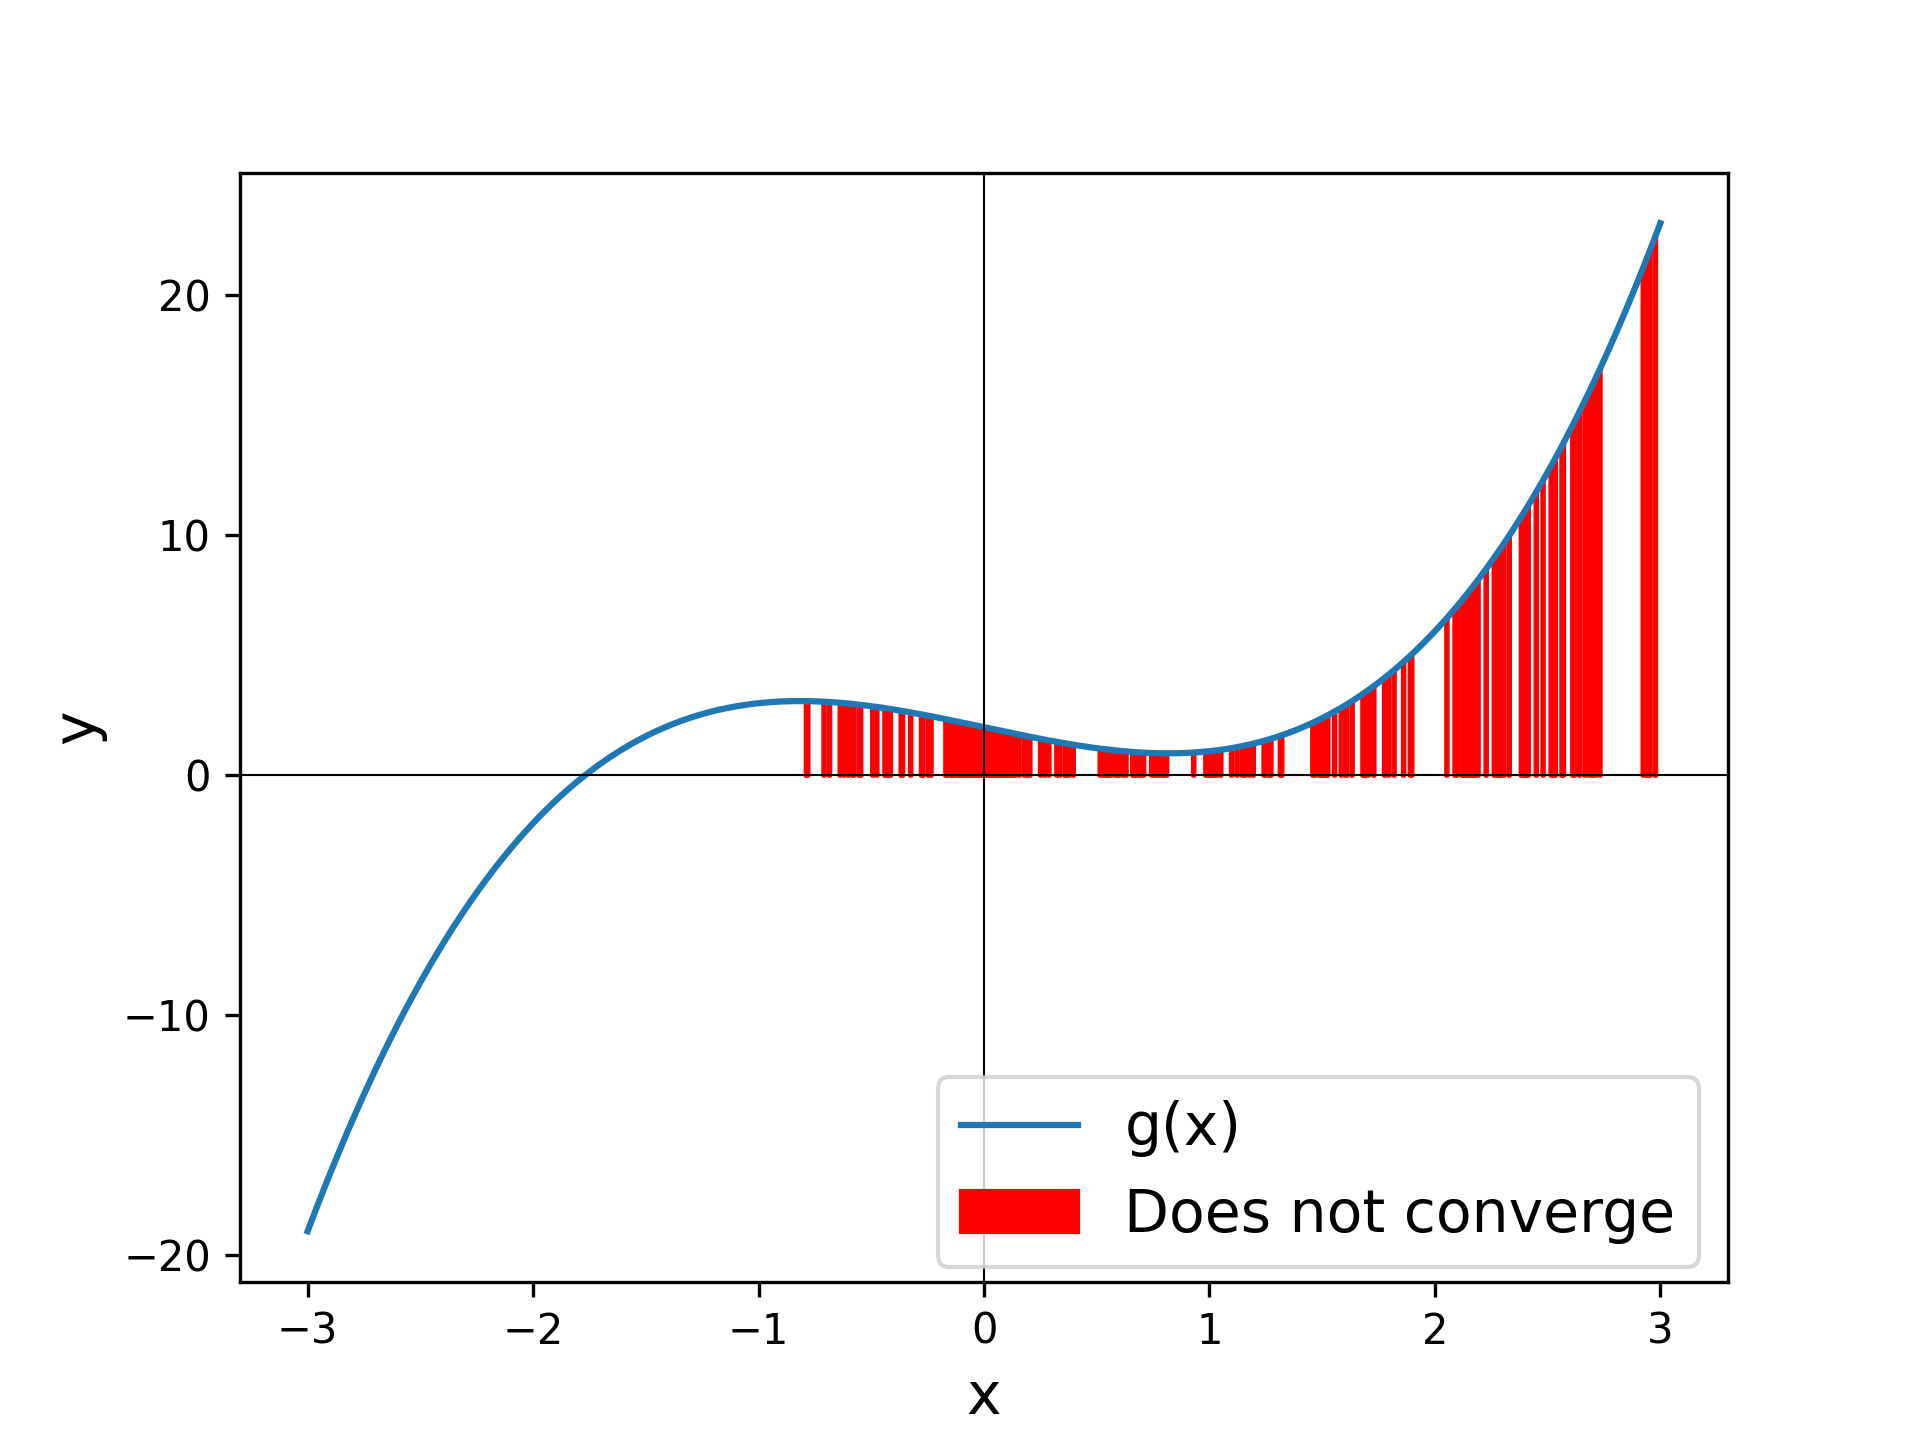
\includegraphics[scale=0.75]{figure1}
		\end{figure}
		\subsection{Diverges}
	
	\section{Basins of Attraction}
	For a given root $ f(x_\star) = 0$, the \emph{basin of attraction} is the set of starting values $ x_0 $ for which Newton's Method will converge to $ x_\star $.
	
		\subsection{Real-Valued Functions}
		Consider the function $ g(x) = (x - 1)(x + 3) $
		\begin{figure}[H]
			\caption{Basins of convergence for $g(x) = (x - 1)(x + 3)$}
			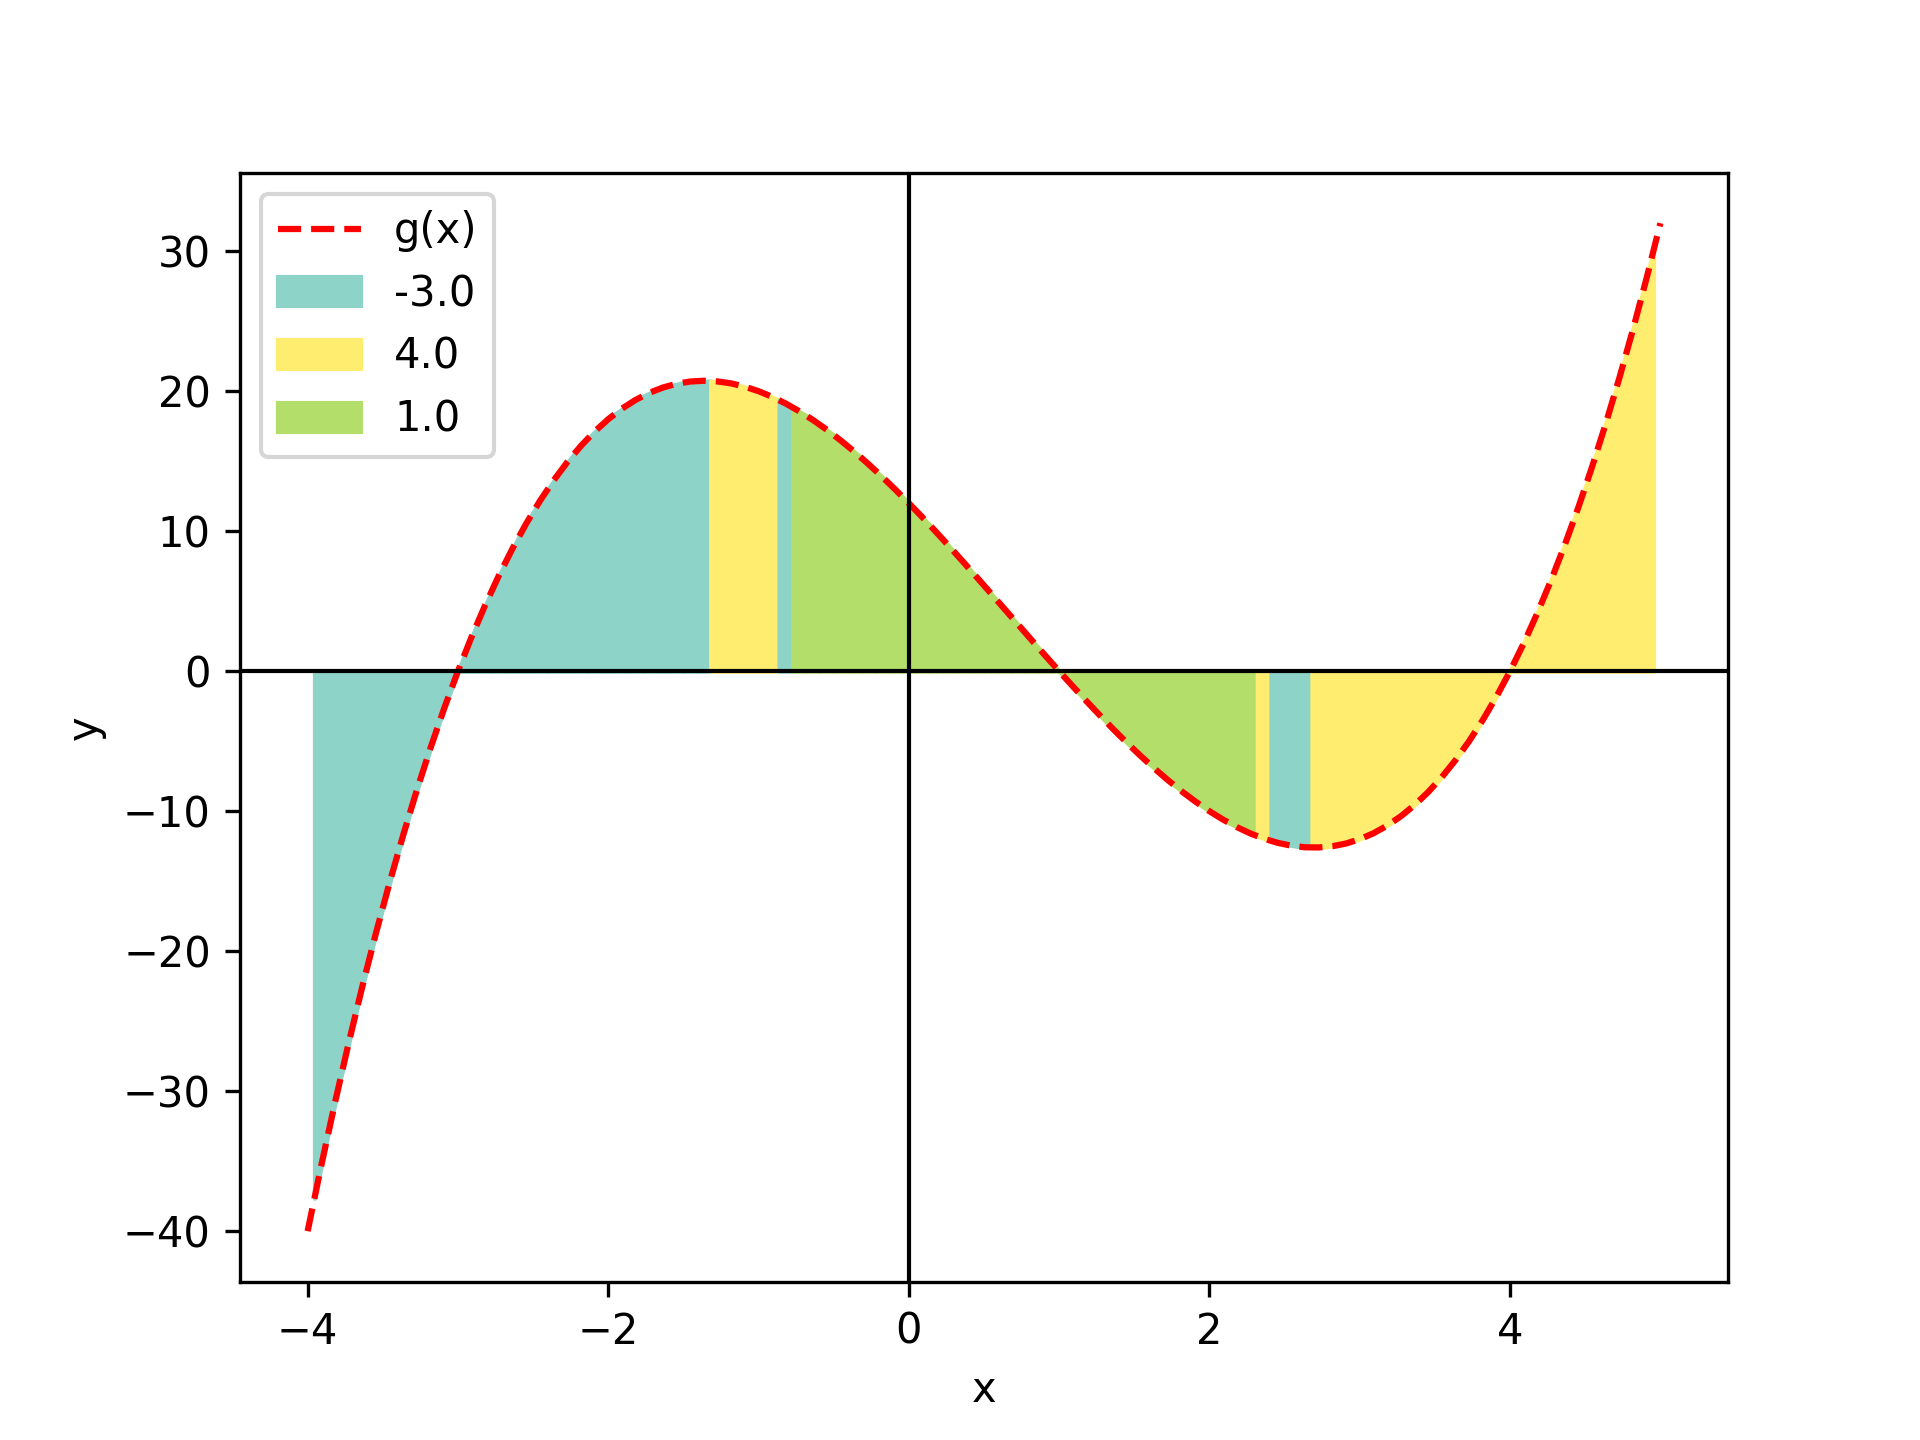
\includegraphics[scale=0.75]{figure2}
		\end{figure}
	
		
		Consider the function $ h(x) =  (x - 4)(x - 1)(x + 3)$
		\begin{figure}[H]
			\caption{Basins of convergence for $h(x) = (x - 4)(x - 1)(x + 3)$}
			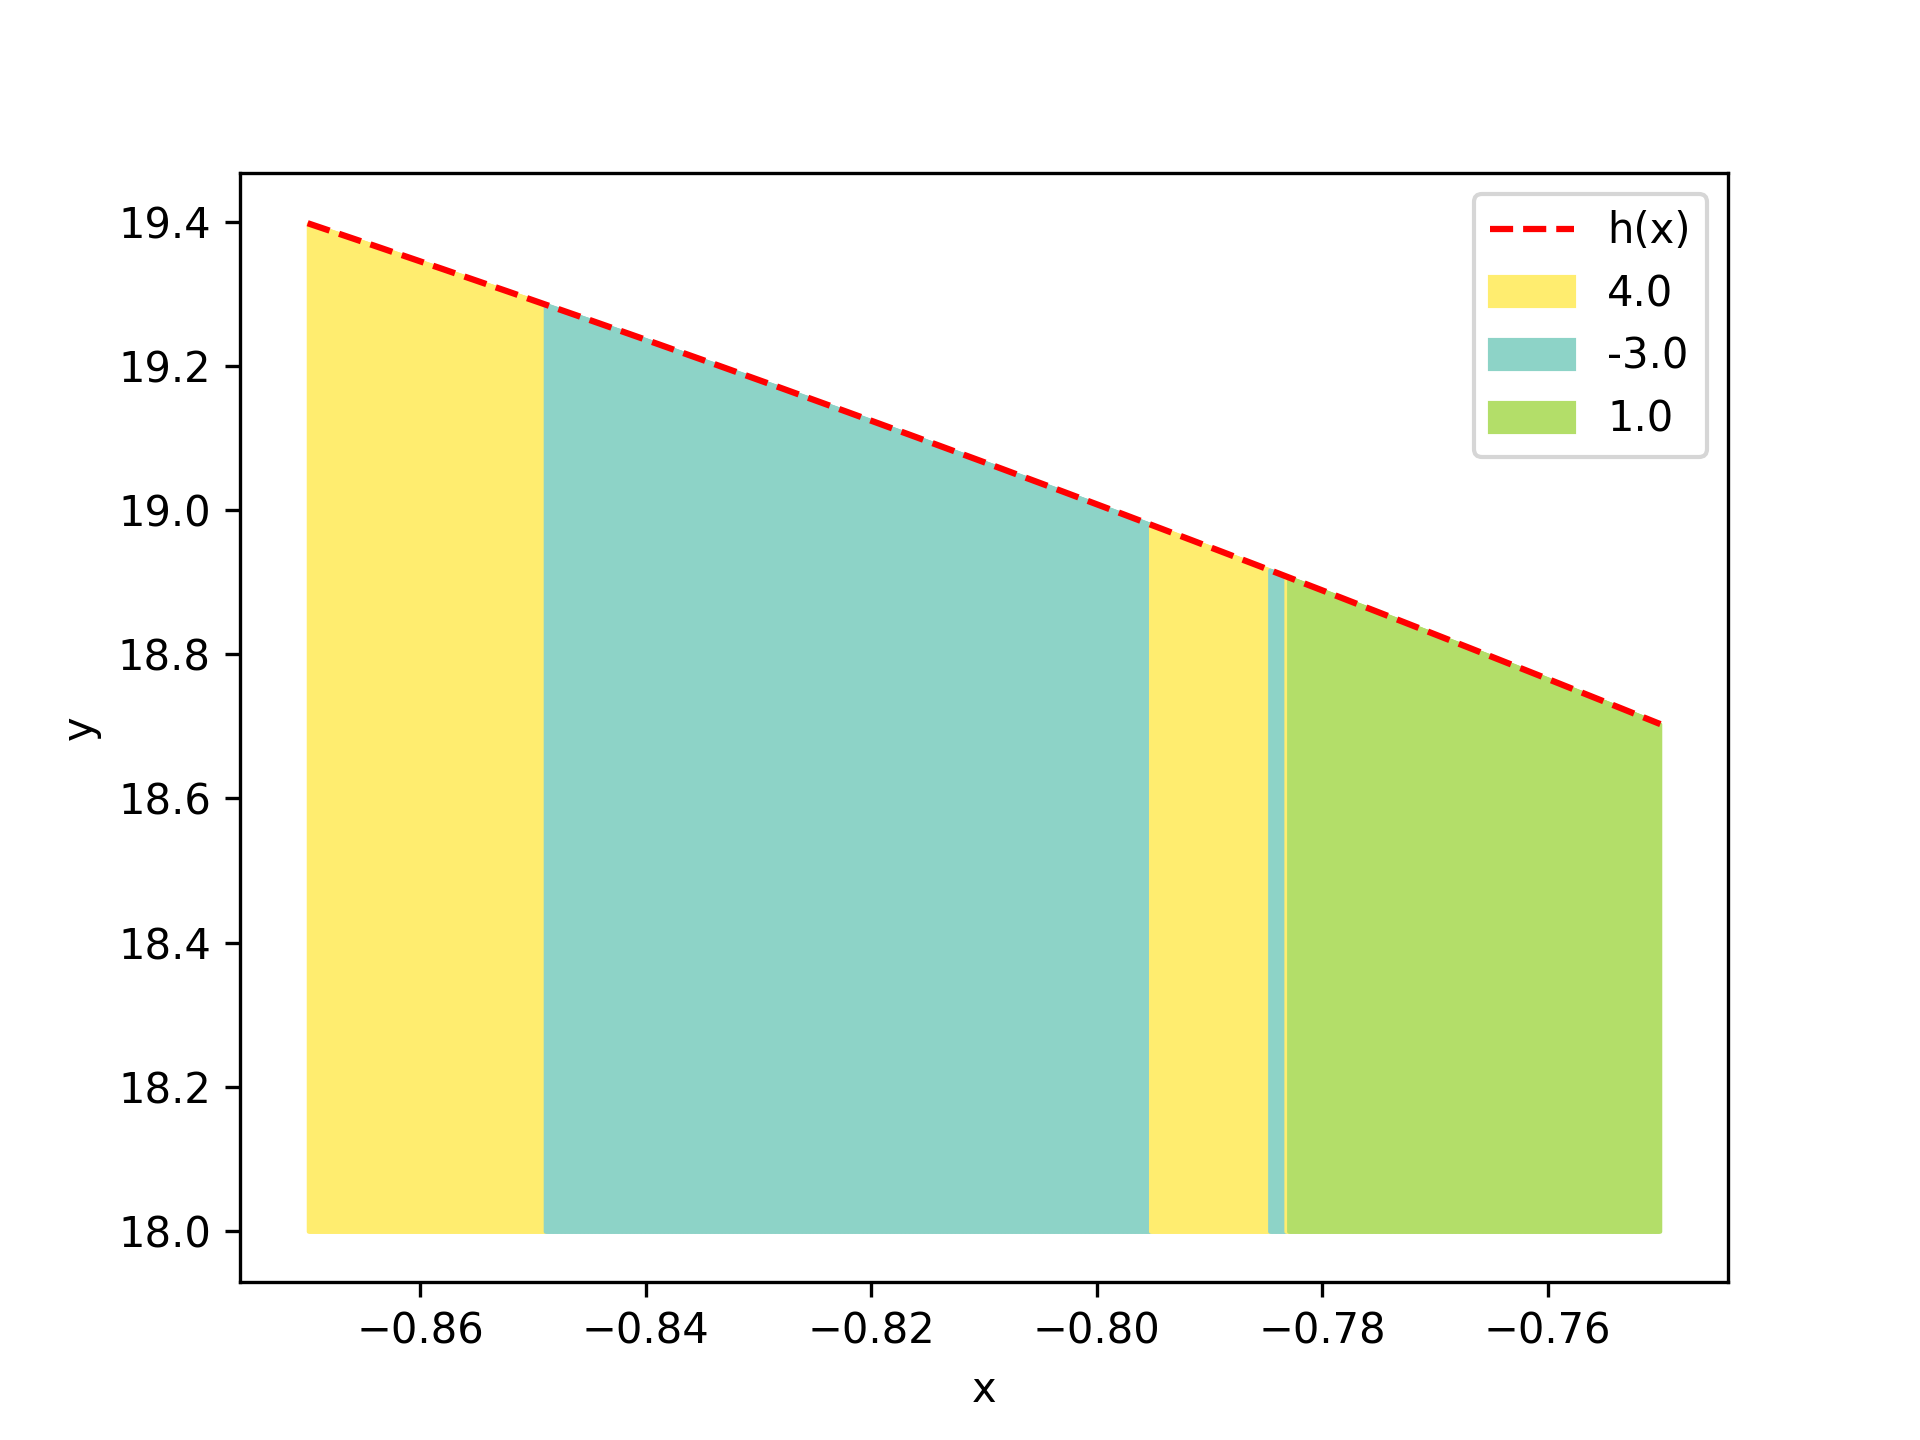
\includegraphics[scale=0.75]{figure3}
		\end{figure}
	
		\begin{figure}[H]
			\caption{Zooming in shows the fractal pattern of the basins}
			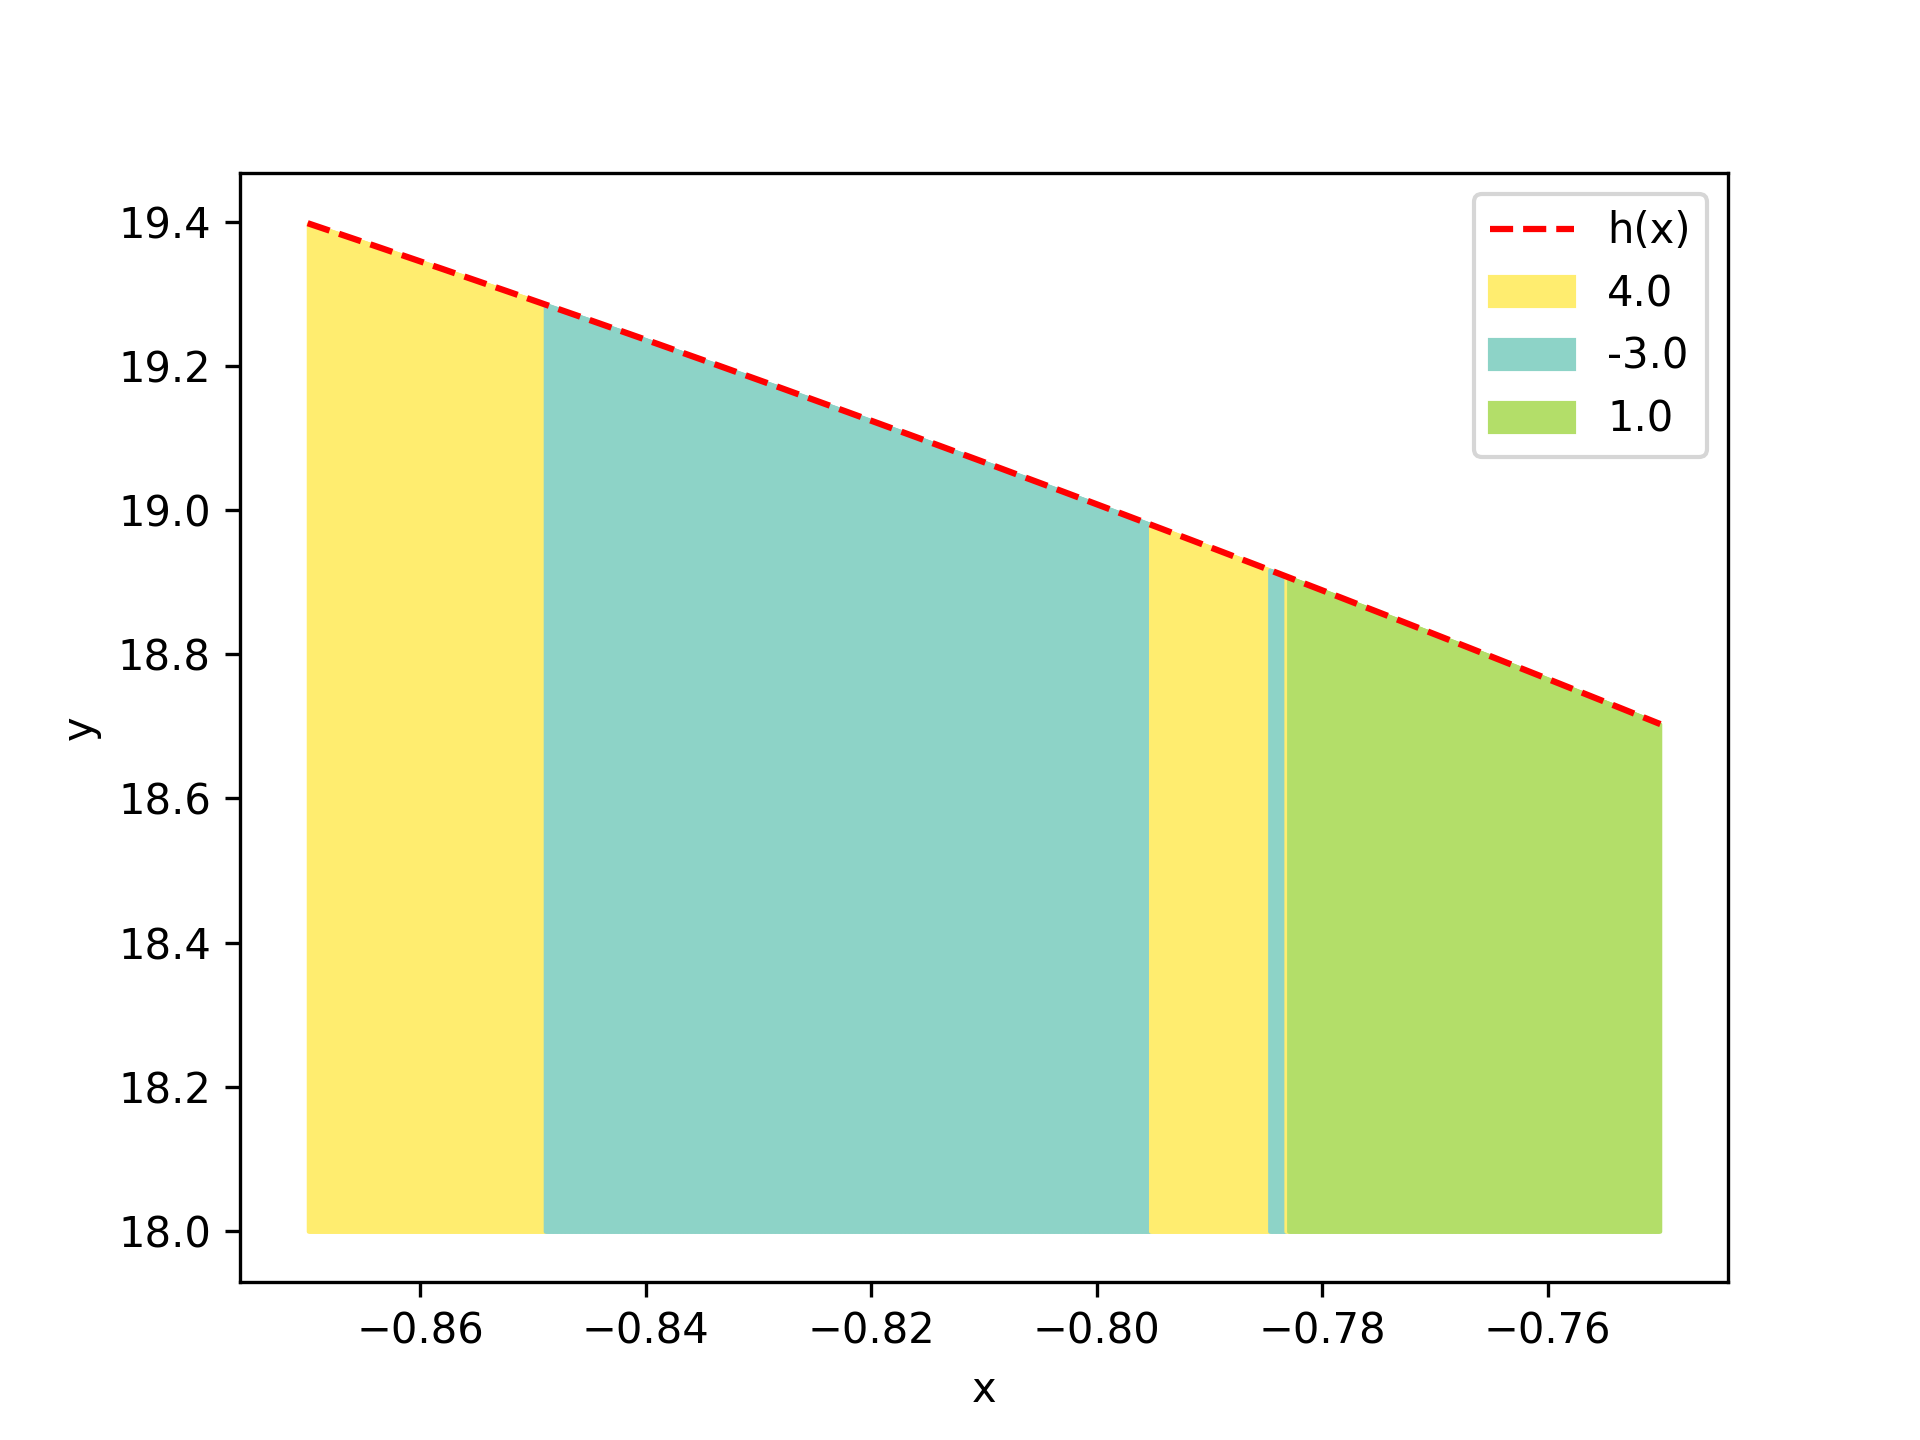
\includegraphics[scale=0.75]{figure4}
		\end{figure}
	
		\subsection{Complex-Valued Functions}
		The fractal behavior of the basins visible in Figure 4 becomes much more intricate when visualized on the complex plane
		\begin{figure}[H]
			\caption{Basins of convergence for $f(z) = z^3 - 1$ on the complex plane $a+bi$}
			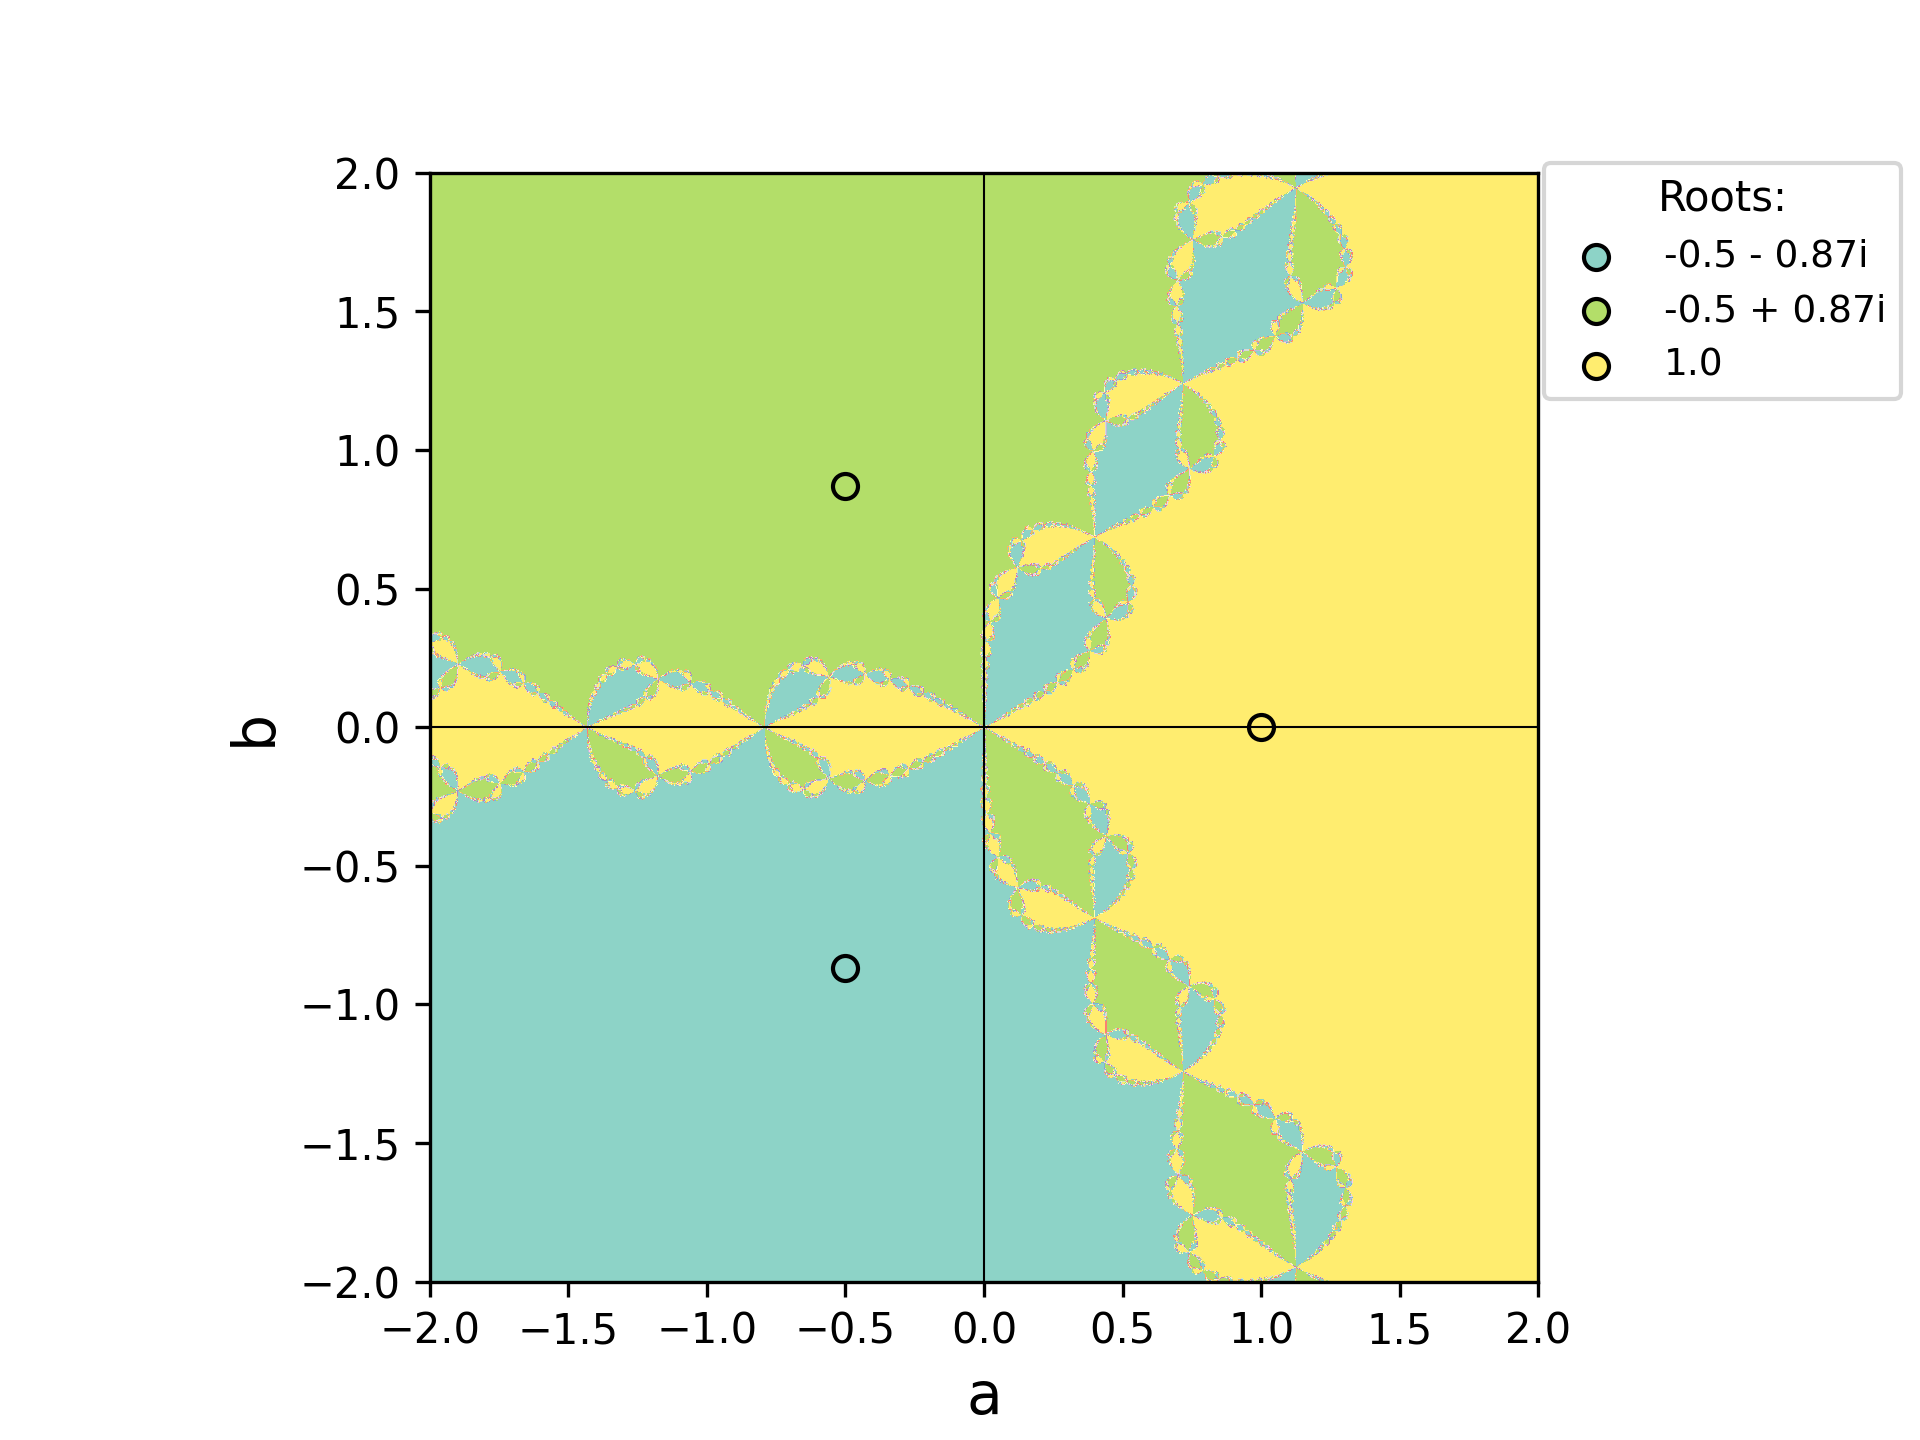
\includegraphics[scale=0.75]{figure5}
		\end{figure}
	
		\begin{figure}[H]
			\caption{Basins of convergence for $g(z) =$ on the complex plane $a+bi$}
			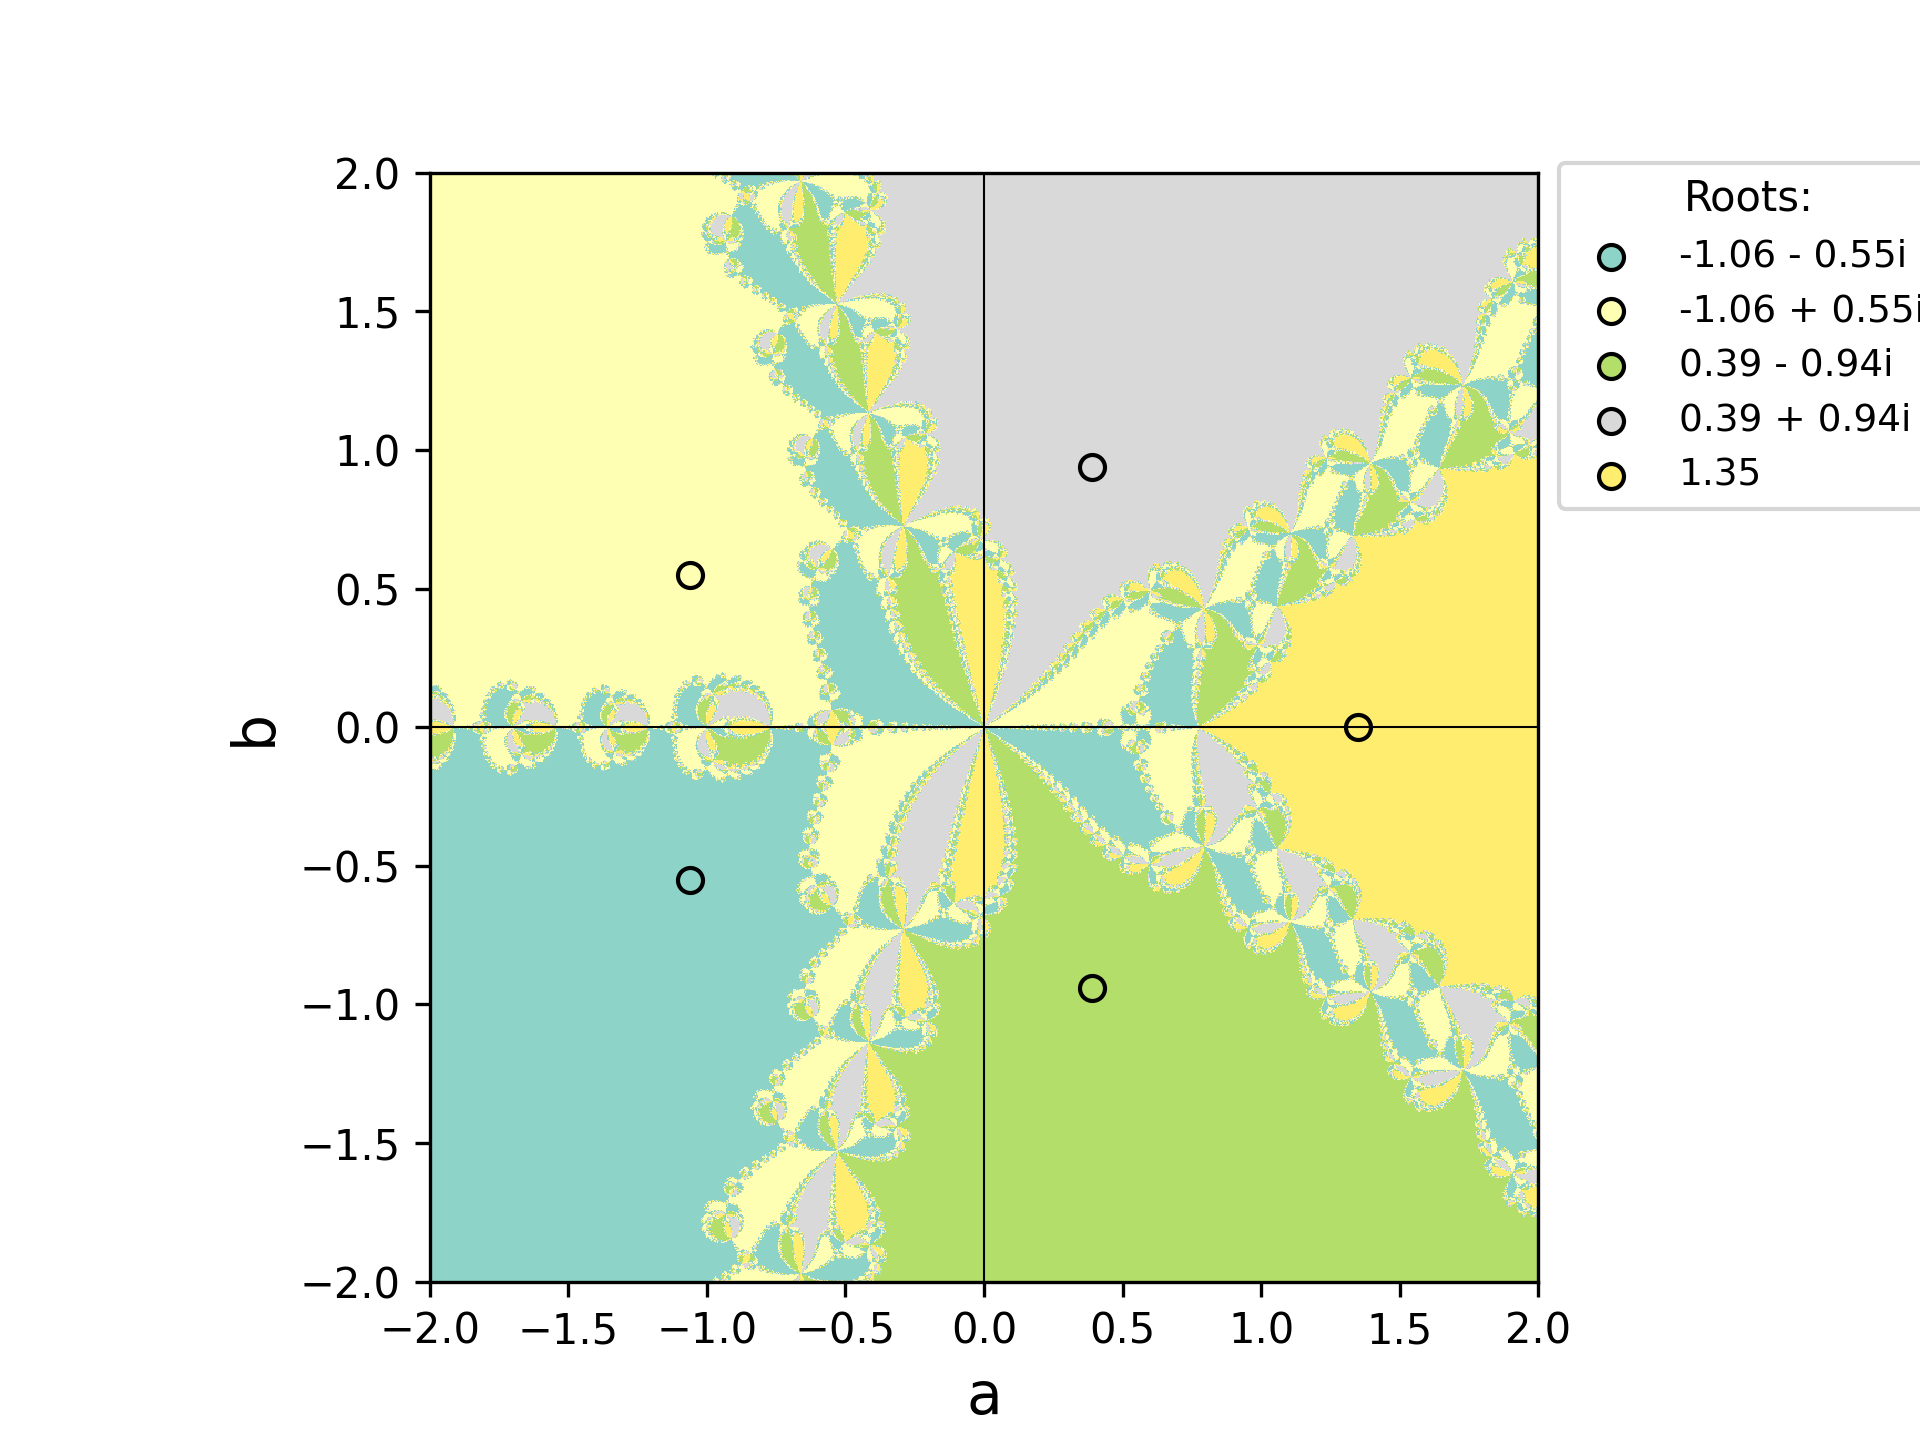
\includegraphics[scale=0.75]{figure6}
		\end{figure}
		

		
	\section{Discussion}
\end{document}